\section{Exploring $k$-Hop Similarity in GNNs}
\subsection{Definition and Properties}

As explained earlier, two graphs $G_1$ and $G_2$ are said to be $k$-hop similar if, for every node in $G_1$, there exists a corresponding node in $G_2$ such that their $k$-hop neighborhoods are identical. Here, the $k$-hop neighborhood of a node includes all nodes reachable within $k$ hops. This concept differs from $k$-hop isomorphism in that the exact connectivity between nodes within the $k$-hop neighborhoods is not required to match.

\begin{figure}[H]
\vskip 0.2in
\begin{center}
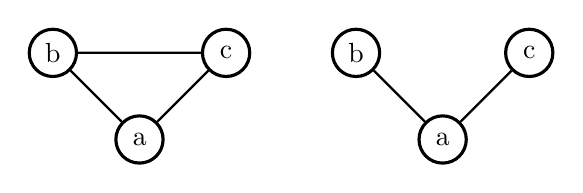
\begin{tikzpicture}[scale=1.1]

% First graph (a-b-c-a)
\node[circle, draw, minimum size=0.6cm, inner sep=0pt, line width=0.4mm] (a1) at (0, 1) {b};
\node[circle, draw, minimum size=0.6cm, inner sep=0pt, line width=0.4mm] (b1) at (2, 1) {c};
\node[circle, draw, minimum size=0.6cm, inner sep=0pt, line width=0.4mm] (c1) at (1, 0) {a};

\draw[thick] (a1) -- (b1);
\draw[thick] (b1) -- (c1);
\draw[thick] (c1) -- (a1);

% Second graph (b-a-c) with reduced space
\node[circle, draw, minimum size=0.6cm, inner sep=0pt, line width=0.4mm] (b2) at (3.5, 1) {b};
\node[circle, draw, minimum size=0.6cm, inner sep=0pt, line width=0.4mm] (a2) at (5.5, 1) {c};
\node[circle, draw, minimum size=0.6cm, inner sep=0pt, line width=0.4mm] (c2) at (4.5, 0) {a};

\draw[thick] (a2) -- (c2);
\draw[thick] (c2) -- (b2);
\end{tikzpicture}
    \end{center}
    \caption{Example of two graphs that are $2$-hop similar but not $2$-hop isomorphic. The left graph shows a complete connection between nodes $a$, $b$, and $c$, while the right graph has the same nodes connected in a path configuration.}
    \label{fig:two_hop_iso}
\end{figure}
To better understand this, consider the example in Figure \ref{fig:two_hop_iso}. Graph 1 and Graph 2 have identical 2-hop neighborhoods for their respective nodes; however, the induced subgraphs (consisting of nodes within 2 hops and the edges between them) for node ``$a$'' are not isomorphic\footnote{The left graph will induce a complete connection between nodes $a$, $b$, and $c$, while the right graph has the same nodes connected in a path configuration.}. Indeed, $k$-hop isomorphism implies $k$-hop similarity, as the latter requires only matching $k$-hop neighborhoods without enforcing identical edge connectivity within these neighborhoods.

\begin{proposition}[\textbf{Isomorphism Implies Similarity}] If two graphs are $k$-hop isomorphic, they are necessarily $k$-hop similar, but the reverse is not always true. \end{proposition}

An alternative interpretation of $k$-hop similarity is that $G_1$ and $G_2$ are considered $k$-hop similar if they can be viewed as $k$-th roots of the same graph $G$. In other terms, $G$ is the $k$-th power graph of both graphs $G1$ and $G_2$.

\begin{definition}[\textbf{$k$-th Power of a Graph}] 
The $k$-th power of a graph $G = (V, E)$, denoted $G^k$, is a graph where there is an edge between nodes $u$ and $v$ if and only if the shortest path distance between them in $G$ is at most $k$. 
\end{definition}

This leads to a practical test for $k$-hop similarity: $G_1$ and $G_2$ are $k$-hop similar if and only if their $k$-th power graphs are identical.

\begin{proposition}[\textbf{Binary $k$-Hop Reachability}]Let $\mathbf{A}_1$ and $\mathbf{A}_2$ be the adjacency matrices of $G_1$ and $G_2$, respectively. Then $G_1$ and $G_2$ are $k$-hop similar if and only if their binary $k$-hop reachability matrices satisfy:
$$R_1 = R_2,$$
where the binary $k$-hop reachability matrix $R_i$ is defined as $R_i = (A_1 + A_i^2 + \cdots + A_i^k > 0)$.
\end{proposition}

Now, the key question arises: how can we generate $k$-hop similar graphs, as we will need them to validate our hypothesis? Intuitively, one might consider computing the $k$-th power graph and then finding its roots. However, this approach is computationally challenging.

\begin{theorem}[\textbf{NP-Hardness}] Computing the roots of the $k$-th power graph is NP-hard.\end{theorem}

\subsection{Constructing $k$-Hop Similar Graphs}
Rather than directly computing the roots of the $k$-th power graph for a given input graph, we propose perturbing the original graph by removing edges, while preserving $k$-hop similarity. To achieve this, we focus on non-critical edges, which we define as edges that do not impact the $k$-hop neighborhoods of the graph.

Specifically, we aim to remove existing edges in such a way that the $k$-hop neighborhoods remain unchanged. To verify that the $k$-hop similarity is preserved, we use the distance matrix, which provides the shortest path distance between any two nodes. If two nodes are within a distance of $k$, we ensure that the operation does not increase the distance beyond $k$. Similarly, if the distance between two nodes is greater than $k$, our operation should not reduce it to less than $k$. To compute the distance matrix, we employ the Floyd-Warshall algorithm.  Algorithm \ref{alg:khopbasic} summarizes our procedure.
\begin{algorithm}[H]
\caption{Generate $K$-Hop Similar Graph}
\label{alg:khopbasic}
\begin{algorithmic}[1]
\REQUIRE{Adjacency matrix $A$, hop count $k$}
\ENSURE{A $k$-hop similar graph $G_{k}$}

\STATE $E \gets \textsc{GetEdges}(A)$
\STATE $G_{k} \gets A$ \hfill $\triangleright$ Copy of adjacency matrix
\STATE $D \gets \textsc{FloydWarshall}(G_{k})$
\STATE $paths_{k} \gets [D \leq k]$ \hfill $\triangleright$ $k$-hop paths

\FOR{each edge $(i,j)$ in $E$}
    \STATE $G_{temp} \gets G_{k}$ \hfill Temporary copy of current graph
    \STATE $G_{temp}[i,j] \gets 0$
    \STATE $G_{temp}[j,i] \gets 0$
    
    \STATE $D_{temp} \gets \textsc{FloydWarshall}(G_{temp})$
    \STATE $paths_{temp} \gets  [D_{temp} \leq k]$
    
    \IF{$paths_{temp} = paths_{k}$}
        \STATE $G_{k}[i,j] \gets 0$
        \STATE $G_{k}[j,i] \gets 0$
        \STATE $D \gets D_{temp}$
    \ENDIF
    
\ENDFOR

\STATE \textbf{return} $G_{k}$
\end{algorithmic}
\end{algorithm}

However, the complexity of this algorithm is quite high, which makes it impractical for very large graphs. The complexity arises from the need to traverse the edge set $E$ for edge removal, and for each edge traversal, compute the distance matrix using Floyd-Warshall \cite{floyd_warshall}, which has a time complexity of $O(V^3)$, where $V$ is the number of vertices. Thus, resulting in an overall complexity of $O(E \times V^3)$.

To address this high complexity, we propose the following modifications:

\begin{enumerate}
    \item \textbf{Threshold on Removals}: We introduce a threshold on the number of edges to remove. The goal is to ensure that the generated graph is structurally different from the original graph. A common measure of structural difference is the graph edit distance, which counts the minimum number of operations required to transform one graph into another. In our case, this would correspond to the number of edges we removed. We define the threshold on the graph edit distance, and once this threshold is reached, we stop exploring further edge modifications.

    \item \textbf{Batching Edge Modifications}: Instead of modifying one edge at a time, we can perform edge removals in batches. This reduces the number of edge traversals and the number of times the distance matrix needs to be recomputed. By processing multiple edges in a single step, we can significantly reduce the overall computational complexity.
\end{enumerate}

\begin{algorithm}[H]
\caption{Generate K-Hop Similar Graph with Batch Processing and Removal Thresholding}
\label{alg:improved_khop}
\begin{algorithmic}[1]
\REQUIRE{Adjacency matrix $A$, hop count $k$, removal threshold $T$, batch size $b$}
\ENSURE{A $k$-hop similar graph $G_k$}
\STATE $(E \gets \textsc{GetEdges}(A)$ \hfill $\triangleright$ Get edge and complementary lists
\STATE $G_{k} \gets A$ \hfill $\triangleright$ Copy of adjacency matrix
\STATE $D \gets \textsc{FloydWarshall}(G_{k})$
\STATE $path_{k} \gets [D\leq k]$ \hfill $\triangleright$$k$-hop paths
\STATE $removals \gets 0$
\FOR{$start \gets 0$ to $|E|$ step $b$}
    \STATE $batch \gets E[start:start+b]$ \hfill $\triangleright$Get current batch of edges
    \STATE $G_{temp} \gets G_{k}$ \hfill $\triangleright$ Temporary copy of current graph
    \FOR{each edge $(i,j)$ in $batch$}
        \STATE $G_{temp}[i,j] \gets 0$
        \STATE $G_{temp}[j,i] \gets 0$
    \ENDFOR  
    \STATE $D_{temp} \gets \textsc{FloydWarshall}(G_{temp})$
    \STATE $path_{temp} \gets [D_{temp} \leq k]$
    \IF{$path_{temp} = path_{k}$}
        \FOR{each edge $(i,j)$ in $batch$}
            \STATE $G_{k}[i,j] \gets 0$
            \STATE $G_{k}[j,i] \gets 0$
        \ENDFOR
        \STATE $D \gets D_{temp}$
        \STATE $removals \gets removals + |batch|$
    \ENDIF   
    \IF{$removals \geq T$}
        \STATE \textbf{return} $G_{k}$
    \ENDIF
\ENDFOR
\STATE \textbf{return} $G_{k}$
\end{algorithmic}
\end{algorithm}
By introducing these modifications, we aim to reduce the time complexity of Algorithm \ref{alg:khopbasic} while maintaining the core objective of perturbing the graph without violating $k$-hop similarity. The threshold on removals controls structural changes by limiting edge modifications, while batching improves efficiency by grouping operations, thus reducing the number of distance matrix computations. The resulting complexity of $O\left(\frac{T \times V^3}{b}\right)$ significantly improves efficiency for larger graphs, where $T$ is the number of edges to modify, $b$ is the batch size and $V$ is the number of nodes. Algorithm \ref{alg:improved_khop} provides a  summary of our approach for constructing $k$-hop similar graphs.

\subsection{Conjecture Validation}
In this section, we conduct a series of experiments to validate our conjecture. To evaluate it across different graph structures, we focus on node classification using synthetic datasets generated with Stochastic Block Models (SBMs) \cite{stochastic_block_models}. SBMs provide a controlled environment for analyzing the influence of structural properties and closely resemble community-structured real-world networks, making them a suitable benchmark for studying the impact of graph structure on our conjecture validity.

After training the GNNs, we validate our conjecture by measuring the level of disagreement between the learned functions trained on two $k$-hop similar graphs. By quantifying disagreement, we aim to understand the sensitivity of learned representations to local structural changes. 

In this context, we define the level of disagreement as: 
\begin{definition}[\textbf{Level of Disagreement}]
The level of disagreement measures the fraction of nodes where the predictions differ between the original graph $ G_1 $ and the $k$-hop similar graph $ G_2 $. Formally:
\[
\text{Disagreement} = \frac{1}{N} \sum_{i=1}^N \mathbb{I}(\hat{y}_i^{(1)} \neq \hat{y}_i^{(2)}),
\]
where:
\begin{itemize}
    \item $ \hat{y}_i^{(1)} $ and $ \hat{y}_i^{(2)} $ are the predicted labels for node $ i $ in $ G_1 $ and $ G_2 $, respectively,
    \item $ \mathbb{I}(\cdot) $ is the indicator function,
    \item $ N $ is the total number of nodes.
\end{itemize}
\end{definition}
\subsubsection{Synthetic Dataset Generation}
We conduct node classification experiments on synthetic graphs generated using stochastic block models (SBMs) to analyze the sensitivity of our assumptions to variations in graph structure. Our base configuration consists of $1500$ nodes, intracluster edge probability of $0.5$, intercluster edge probability of $0.1$, and $2$ classes. To isolate the influence of each parameter, we perform controlled experiments where we fix all other parameters and vary one at a time. Specifically, we vary the number of nodes between $50$ and $3000$, intra-cluster edge probability between $0.1$ and $0.9$, inter-cluster edge probability between $0.1$ and $0.9$, and the number of classes between $2$ and $10$.

Node features are sampled from a $1024$-dimensional Gaussian distribution, where each class has a unique mean vector equal to its class label, and variance is set to $1$. The dataset is approximately balanced, with an equal number of nodes per class. We use a $80/20/20$ split for training, validation, and testing, respectively
 
\subsubsection{Experimental Setting}
For $k$-hop similar graph generation, we use Algorithm \ref{alg:improved_khop} and set the graph edit distance threshold to $20\%$ of the edges in the original input graph. The batch size is chosen such that it corresponds to half of the edges to be removed. This ensures a trade-off between generating diverse graph structures while maintaining $k$-hop similarity to the original graph.

We train a two-layer Graph Convolutional Neural Network (GCN) \cite{kipf2017semisupervisedclassificationgraphconvolutional} with ReLU activation, and $32$ hidden units.

All models are trained using the Adam optimizer \cite{kingma2017adammethodstochasticoptimization}  with a learning rate of 0.01 for up to $200$ epochs. Early stopping is applied based on validation loss, using a window size of $50$ epochs. Performance is evaluated using accuracy and the level of disagreement across all datasets. 

All experimental results are averaged over $10$ independent runs with different random initializations to ensure statistical robustness, reporting both mean and standard deviation (mean $\pm$ std).


\subsubsection{Numerical Results}
\paragraph{Number of nodes.}
Table \ref{tab:number_nodes} compares the performance of the model on original and $k$-hop similar graphs with varying node counts (ranging from $50$ to $3,000$). The results strongly validate the weight consistency conjecture, showing that $ f_{\theta_1} \approx f_{\theta_2} $ holds for different graph scales. This is reflected in the exceptionally low disagreement rates ($\leq 0.69\%$) and nearly identical accuracy scores between graph pairs, despite notable structural differences ($20\%$ edges are different).
\begin{table}[H]
\caption{Performance comparison across different number of nodes. Results show classification accuracy (\%) on original and $K$-hop similar graphs, and level of disagreement (\%). All metrics are reported as mean $\pm$ standard deviation over $10$ runs.}
\label{tab:number_nodes}
\vskip 0.15in
\begin{center}
\resizebox{0.6\columnwidth}{!}{
\begin{small}
\begin{sc}
\begin{tabular}{r|ccc}
\toprule
\textbf{Nodes} & \textbf{Original Graph Acc.} & \textbf{K-Hop Graph Acc.} & \textbf{Disagreement} \\
\midrule
50 & 94.00 $\pm$ 18.00 & 94.00 $\pm$ 18.00 & 0.20 $\pm$ 0.60  \\
100 & 100.00 $\pm$ 0.00 & 100.00 $\pm$ 0.00 & 0.00 $\pm$ 0.00  \\
500 & 92.40 $\pm$ 3.35 & 92.20 $\pm$ 2.56 & 0.32 $\pm$ 0.39  \\
1000 & 98.45 $\pm$ 2.81 & 97.75 $\pm$ 3.24 & 0.69 $\pm$ 1.06 \\
1500 & 99.97 $\pm$ 0.10 & 99.97 $\pm$ 0.10 & 0.06 $\pm$ 0.18 \\
2000 & 98.65 $\pm$ 2.64 & 98.67 $\pm$ 2.65 & 0.02 $\pm$ 0.03  \\
2500 & 99.26 $\pm$ 2.22 & 99.26 $\pm$ 2.22 & 0.00 $\pm$ 0.00  \\
3000 & 100.00 $\pm$ 0.00 & 100.00 $\pm$ 0.00 & 0.00 $\pm$ 0.00  \\
\bottomrule
\end{tabular}
\end{sc}
\end{small}
}
\end{center}
\vskip -0.1in
\end{table}


\paragraph{Intracluster Probability.}

Table \ref{tab:intraclass_performance} explores the effect of varying intra-class connection probabilities (ranging from $0.2$ to $0.9$) on the consistency of the learned functions. The results strongly support $ f_{\theta_1} \approx f_{\theta_2} $, showing extremely low disagreement rates ($\leq 0.25\%$) and negligible differences in accuracy (maximum of $0.03\%$) between original and $k$-hop similar graphs. This consistency holds across all values of intraclass probability, implying that the learned functions remain largely unchanged regardless of the density of connections within the same class.
\begin{table}[H]
\caption{Performance comparison across different intraclass probability values. Results show classification accuracy (\%) on original and $K$-hop similar graphs, and level of disagreement (\%). All metrics are reported as mean $\pm$ standard deviation over $10$ runs.}
\label{tab:intraclass_performance}
\vskip 0.15in
\begin{center}
\resizebox{0.6\columnwidth}{!}{
\begin{small}
\begin{sc}
\begin{tabular}{r|ccc}
\toprule
\textbf{Intra-Class} & \textbf{Original Graph Acc.} & \textbf{K-Hop Graph Acc.} & \textbf{Disagreement} \\
\textbf{Probability} & \textbf{(\%)} & \textbf{(\%)} & \textbf{(\%)} \\
\midrule
0.2 & 88.77 $\pm$ 1.54 & 88.77 $\pm$ 1.54 & 0.00 $\pm$ 0.00 \\
0.3 & 90.80 $\pm$ 8.98 & 90.77 $\pm$ 9.07 & 0.25 $\pm$ 0.34 \\
0.4 & 99.50 $\pm$ 1.50 & 99.53 $\pm$ 1.40 & 0.03 $\pm$ 0.08 \\
0.5 & 99.40 $\pm$ 1.80 & 99.43 $\pm$ 1.70 & 0.05 $\pm$ 0.14 \\
0.6 & 97.77 $\pm$ 3.48 & 97.73 $\pm$ 3.51 & 0.02 $\pm$ 0.03 \\
0.7 & 98.97 $\pm$ 2.07 & 99.00 $\pm$ 2.01 & 0.07 $\pm$ 0.22 \\
0.8 & 100.00 $\pm$ 0.00 & 100.00 $\pm$ 0.00 & 0.00 $\pm$ 0.00 \\
0.9 & 100.00 $\pm$ 0.00 & 100.00 $\pm$ 0.00 & 0.00 $\pm$ 0.00 \\
\bottomrule
\end{tabular}
\end{sc}
\end{small}
}
\end{center}
\vskip -0.1in
\end{table}


\paragraph{Intercluster Probability.}
Table \ref{tab:interclass_performance} investigates the impact of varying interclass connection probabilities (from $0$ to $0.9$) on function consistency. Although the overall accuracy decreases with higher interclass connectivity, the approximation $ f_{\theta_1} \approx f_{\theta_2} $ remains strong, as evidenced by low disagreement rates ($\leq 0.51\%$) and consistent accuracy scores (maximum difference of $0.32\%$). This suggests that the weight consistency conjecture continues to hold even as the graph structure becomes more complex with increased interclass connectivity.
\begin{table}[H]
\caption{Performance comparison across different interclass probability values. Results show classification accuracy (\%) on original and $K$-hop similar graphs, and level of disagreement (\%). All metrics are reported as mean $\pm$ standard deviation over $10$ runs.}
\label{tab:interclass_performance}
\vskip 0.15in
\begin{center}
\resizebox{0.6\columnwidth}{!}{
\begin{small}
\begin{sc}
\begin{tabular}{r|ccc}
\toprule
\textbf{Inter-Class} & \textbf{Original Graph Acc.} & \textbf{K-Hop Graph Acc.} & \textbf{Disagreement} \\
\textbf{Probability} & \textbf{(\%)} & \textbf{(\%)} & \textbf{(\%)} \\
\midrule
0.0 & 100.00 $\pm$ 0.00 & 100.00 $\pm$ 0.00 & 0.00 $\pm$ 0.00 \\
0.1 & 99.60 $\pm$ 1.60 & 99.92 $\pm$ 0.30 & 0.28 $\pm$ 1.12 \\
0.2 & 99.73 $\pm$ 1.32 & 99.94 $\pm$ 0.24 & 0.20 $\pm$ 0.92 \\
0.3 & 92.57 $\pm$ 13.23 & 92.47 $\pm$ 13.67 & 0.51 $\pm$ 1.22 \\
0.4 & 86.91 $\pm$ 16.47 & 86.83 $\pm$ 16.73 & 0.41 $\pm$ 1.11 \\
0.5 & 83.68 $\pm$ 16.70 & 83.61 $\pm$ 16.90 & 0.34 $\pm$ 1.02 \\
0.6 & 80.72 $\pm$ 17.11 & 80.66 $\pm$ 17.27 & 0.30 $\pm$ 0.96 \\
0.7 & 78.55 $\pm$ 17.04 & 78.49 $\pm$ 17.17 & 0.26 $\pm$ 0.90 \\
0.8 & 76.87 $\pm$ 16.78 & 76.83 $\pm$ 16.89 & 0.23 $\pm$ 0.85 \\
0.9 & 75.66 $\pm$ 16.35 & 75.62 $\pm$ 16.46 & 0.21 $\pm$ 0.81 \\
\bottomrule
\end{tabular}
\end{sc}
\end{small}
}
\end{center}
\end{table}

\paragraph{Number of classes.}
Table \ref{tab:classes_performance} reveals a surprising behavior when examining the weight consistency conjecture across different numbers of classes (ranging from $2$ to $10$). While \( f_{\theta_1} \approx f_{\theta_2} \) holds strongly for binary and three-class problems (with disagreement \(\leq 4.24\%\)), we observe an unexpected sharp increase in disagreement rates for higher numbers of classes, reaching up to $81.08\%$ for $10$ classes. Intriguingly, despite this high disagreement in individual predictions, both models maintain remarkably similar overall accuracy scores (with a maximum difference of $2.47\%$).
\begin{table}[H]
\caption{Performance comparison across different numbers of classes. Results show classification accuracy (\%) on original and $K$-hop similar graphs, and level of disagreement (\%). All metrics are reported as mean $\pm$ standard deviation over $10$ runs.}
\label{tab:classes_performance}
\vskip 0.15in
\begin{center}
\resizebox{0.6\columnwidth}{!}{
\begin{small}
\begin{sc}
\begin{tabular}{r|ccc}
\toprule
\textbf{Number of} & \textbf{Original Graph Acc.} & \textbf{K-Hop Graph Acc.} & \textbf{Disagreement} \\
\textbf{Classes} & \textbf{(\%)} & \textbf{(\%)} & \textbf{(\%)} \\
\midrule
2 & 99.43 $\pm$ 0.86 & 99.00 $\pm$ 1.48 & 0.63 $\pm$ 1.05 \\
3 & 78.27 $\pm$ 7.83 & 77.30 $\pm$ 6.54 & 4.24 $\pm$ 4.54 \\
4 & 72.20 $\pm$ 6.07 & 70.10 $\pm$ 3.49 & 4.30 $\pm$ 4.83 \\
5 & 44.10 $\pm$ 6.05 & 46.57 $\pm$ 9.35 & 45.95 $\pm$ 33.28 \\
6 & 28.87 $\pm$ 8.25 & 28.67 $\pm$ 7.70 & 73.81 $\pm$ 30.42 \\
7 & 29.37 $\pm$ 7.82 & 29.83 $\pm$ 8.11 & 54.43 $\pm$ 35.84 \\
8 & 19.63 $\pm$ 5.01 & 20.30 $\pm$ 4.90 & 78.47 $\pm$ 16.74 \\
9 & 21.17 $\pm$ 2.71 & 21.23 $\pm$ 3.89 & 77.79 $\pm$ 6.88 \\
10 & 17.33 $\pm$ 4.67 & 17.60 $\pm$ 4.82 & 81.08 $\pm$ 20.75 \\
\bottomrule
\end{tabular}
\end{sc}
\end{small}
}
\end{center}
\end{table}
Investigating the predicted class probabilities reveals that this apparent contradiction arises from model uncertainty. As the number of classes increases, the models produce increasingly uniform probability distributions across classes, indicating low confidence in their predictions. This explains why small perturbations in input graphs can lead to different class assignments while maintaining similar accuracy levels: essentially, the models are making near-random choices among equally uncertain options. In other words, while the models may assign different classes due to subtle changes in the input, the lack of clear discrimination between classes results in similar accuracy outcomes. 

\begin{figure}[H]
    \vskip 0.2in
    \begin{center}    \centerline{\includegraphics[width=0.6\columnwidth]{Figures/mean_probs_origin.png}}
    \caption{Average predicted probability distribution across ten classes for a GNN model trained on the original graph.}
    \label{origin}
    \end{center}
    \vskip -0.2in
\end{figure}

\begin{figure}[H]
    \vskip 0.2in
    \begin{center}
    \centerline{\includegraphics[width=0.6\columnwidth]{Figures/mean_probs_origin.png}}
    \caption{Average predicted probability distribution across ten classes for a GNN model trained on the $2$-hop similar graph.}
    \label{hophop}
    \end{center}
    \vskip -0.2in
\end{figure}

Figures \ref{origin} and \ref{hophop} present the average predicted probability distribution for disagreed nodes across ten classes, comparing the models trained on the original graph and the two-hop similar graph. The near-uniform distribution (with probabilities ranging from approximately 0.08 to 0.10) indicates the model's low confidence in class assignments. Each class receives similar probability mass, regardless of the true label, which suggests that the model is uncertain in distinguishing between the classes.

This behavior suggests that the issue is not with the weight consistency conjecture itself, but rather with the model's fundamental inability to learn discriminative features for multi-class classification tasks. 


Based on our experimental analysis, we consider that Conjecture \ref{conjecture: weight_consistency} is \textbf{valid}.


